\chapter{Le Soleil dans le ciel~: jours et saisons}\label{ch:g3:sun-days-seasons}

En juin, tu joues dehors après le dîner dans une \omterm{def:g1:light-and-shadows:source}{lumière} dorée~; en
décembre, les lampadaires s'allument avant que tu ne rentres de
l'école. Le Soleil garde sa vieille habitude --- il monte d'un côté,
passe au plus haut, redescend de l'autre --- mais sa route à travers
le ciel n'est pas la même toute l'année. Suis-le pendant une année
entière, et tu découvres les \omterm{def:g3:sun-days-seasons:year}{saisons}.

\section{La route changeante du Soleil}

\begin{example}[Route d'été, route d'hiver]\label{ex:g3:sun-days-seasons:roads}
Observe l'arc du Soleil au cœur de l'été~: il se lève tôt, monte très
haut --- presque au-dessus de ta tête à midi --- et se couche tard~:
une route longue et haute, et une longue journée. Au cœur de l'hiver,
l'arc est bas et court~: le Soleil se lève tard, ne monte jamais bien
au-dessus des toits, et se couche au milieu de l'après-midi. Entre
les deux, au printemps et en automne, la route est moyenne --- et le
jour et la nuit se partagent les \omterm{ex:g2:measuring-time:clock}{heures} presque également.
\end{example}

\begin{omfigure}
\begin{tikzpicture}[scale=0.85]
  \draw[thick] (0,0) -- (11,0);
  \draw[dashed, omThm, thick] (1.0,0.2) .. controls (3.5,4.6)
    and (7.5,4.6) .. (10.0,0.2);
  \fill[omThm] (5.5,3.5) circle (0.3);
  \node[above, font=\small, omThm] at (5.5,3.9) {plein été~: haute et longue};
  \draw[dashed, omDef, thick] (2.6,0.15) .. controls (4.4,1.7)
    and (6.6,1.7) .. (8.4,0.15);
  \fill[omDef] (5.5,1.3) circle (0.3);
  \node[above, font=\small, omDef] at (2.9,1.35) {plein hiver~: basse et courte};
\end{tikzpicture}

{\small Les deux routes extrêmes du Soleil au-dessus du même horizon.
Le haut arc d'été demande de nombreuses \omterm{ex:g2:measuring-time:clock}{heures}~; le bas arc d'hiver
est achevé au milieu de l'après-midi.}
\end{omfigure}

\begin{proposition}[La règle de midi]\label{prop:g3:sun-days-seasons:midday}
En toute \omterm{def:g3:sun-days-seasons:year}{saison}, le Soleil est au plus haut au milieu de la journée
--- et à cet instant, chaque \omterm{def:g1:light-and-shadows:shadow}{ombre} est la plus courte de la journée
et pointe dans la même direction que l'\omterm{def:g1:light-and-shadows:shadow}{ombre} de midi d'hier, et que
celle de demain. Les \omterm{def:g1:light-and-shadows:shadow}{ombres} de midi sont les flèches les plus fiables
de la nature.
\end{proposition}

\begin{example}[Lire la saison dans une
ombre]\label{ex:g3:sun-days-seasons:shadowlength}
La \emph{longueur} de l'\omterm{def:g1:light-and-shadows:shadow}{ombre} de midi change avec la \omterm{def:g3:sun-days-seasons:year}{saison}~: en été,
le Soleil étant presque au-dessus de nos têtes, l'\omterm{def:g1:light-and-shadows:shadow}{ombre} de midi d'un
poteau n'est qu'un petit moignon~; en hiver, le Soleil restant bas,
le même poteau jette à midi une longue \omterm{def:g1:light-and-shadows:shadow}{ombre}. Marque une fois par
mois la pointe de l'\omterm{def:g1:light-and-shadows:shadow}{ombre} de midi sur le sol, et les marques
avanceront et reculeront au fil de l'année comme un lent balancier.
\end{example}

\section{L'horloge d'ombre}

\begin{definition}[Cadran solaire]\label{def:g3:sun-days-seasons:sundial}
Un \emph{cadran solaire}\index{cadran solaire} est une horloge faite
d'une \omterm{def:g1:light-and-shadows:shadow}{ombre}~: un bâton ou une lame dressés au soleil, avec des
repères tout autour indiquant où tombe l'\omterm{def:g1:light-and-shadows:shadow}{ombre} à chaque heure. À
mesure que le Soleil parcourt son arc, l'\omterm{def:g1:light-and-shadows:shadow}{ombre} balaie les repères ---
lentement, sans bruit, et sans la moindre pièce mobile.
\end{definition}

\begin{method}[Construire une horloge d'ombre]\label{met:g3:sun-days-seasons:build}
Un matin ensoleillé, à un endroit qui reste au soleil toute la
journée~:
\begin{enumerate}
  \item planter un bâton bien droit dans un sol plat (ou le dresser
        dans un seau de sable)~;
  \item toutes les \omterm{ex:g2:measuring-time:clock}{heures}, à l'heure \omterm{def:g3:first-electric-circuit:battery}{pile}, marquer la pointe de son
        \omterm{def:g1:light-and-shadows:shadow}{ombre} avec un caillou et écrire l'heure dessus à la craie~;
  \item continuer jusqu'au soir.
\end{enumerate}
Demain, l'\omterm{def:g1:light-and-shadows:shadow}{ombre} passera sur tes cailloux à l'heure dite~: ton bâton
donne maintenant l'heure. (Pour un temps, du moins --- comme la
\omterm{def:g3:sun-days-seasons:year}{saison} glisse, les \omterm{def:g1:light-and-shadows:shadow}{ombres} glissent aussi, et tes cailloux se
tromperont peu à peu.)
\end{method}

\begin{omfigure}
\begin{tikzpicture}[scale=0.85]
  \draw[thick] (0.5,0) -- (10.5,0);
  \draw[very thick] (5.5,0) -- (5.5,1.7);
  \draw[line width=3pt, omExo] (5.5,0) -- (2.2,0.9);
  \draw[line width=3pt, omExo, opacity=0.6] (5.5,0) -- (4.1,1.35);
  \draw[line width=3pt, omExo, opacity=0.35] (5.5,0) -- (5.5,1.5);
  \draw[line width=3pt, omExo, opacity=0.6] (5.5,0) -- (6.9,1.35);
  \draw[line width=3pt, omExo] (5.5,0) -- (8.8,0.9);
  \node[font=\footnotesize] at (1.8,1.0) {matin};
  \node[font=\footnotesize] at (5.5,1.9) {midi~: la plus courte};
  \node[font=\footnotesize] at (9.4,1.0) {soir};
\end{tikzpicture}

{\small Un bâton, une journée~: l'\omterm{def:g1:light-and-shadows:shadow}{ombre} balaie comme une aiguille
lente, la plus longue aux deux bords du jour, la plus courte à midi.}
\end{omfigure}

\section{L'année et ses saisons}

\begin{definition}[L'année et les saisons]\label{def:g3:sun-days-seasons:year}
Pendant que la Terre tourne une fois par jour sur elle-même, elle
accomplit aussi un immense voyage \emph{autour du Soleil} --- un tour
complet dure une \emph{année}\index{année}, environ $365$ jours. Au
long de ce tour, la route du Soleil dans notre ciel s'élève puis
s'abaisse lentement, et nous traversons les quatre
\emph{saisons}\index{saison}~: le printemps, l'été, l'automne,
l'hiver --- puis le printemps de nouveau, tour après tour.
\end{definition}

\begin{example}[Les quatre quarts]\label{ex:g3:sun-days-seasons:quarters}
L'été~: Soleil haut, journées longues, \omterm{def:g1:light-and-shadows:shadow}{ombres} de midi courtes.
L'hiver~: Soleil bas, journées courtes, \omterm{def:g1:light-and-shadows:shadow}{ombres} de midi longues. Le
printemps et l'automne se placent entre les deux --- et dans chacun
d'eux arrive un jour particulier où le jour et la nuit durent
exactement autant. Les paysans, les marins et les bâtisseurs d'autrefois
ont appris à lire ce calendrier directement dans le ciel.
\end{example}

\begin{omfigure}
\begin{tikzpicture}[scale=0.85]
  \fill[omThm] (5.5,1.8) circle (0.5);
  \foreach \a in {0,30,...,330} {
    \draw[omThm] (5.5,1.8) ++(\a:0.68) -- ++(\a:0.26);
  }
  \draw[dashed, thick] (5.5,1.8) ellipse (4.4 and 1.55);
  \fill[omDef] (1.1,1.8) circle (0.26);
  \fill[omDef] (9.9,1.8) circle (0.26);
  \fill[omDef] (5.5,3.35) circle (0.26);
  \fill[omDef] (5.5,0.25) circle (0.26);
  \node[left, font=\small] at (0.75,1.8) {ici, l'hiver};
  \node[right, font=\small] at (10.25,1.8) {ici, l'été};
  \node[above, font=\small] at (5.5,3.7) {printemps};
  \node[below, font=\small] at (5.5,-0.1) {automne};
\end{tikzpicture}

{\small Un tour de la Terre autour du Soleil --- une année, quatre
\omterm{def:g3:sun-days-seasons:year}{saisons}. Pourquoi la route basse en hiver et la route haute en été~?
Ce secret est gardé pour un chapitre plus loin, sur la famille
Soleil--Terre--Lune.}
\end{omfigure}

\begin{remark}[L'hiver n'est pas «~plus loin~»]\label{rem:g3:sun-days-seasons:notfarther}
Il est tentant de deviner que l'hiver est froid parce que la Terre
s'éloigne du Soleil. Eh bien non --- la distance ne change presque
pas, et quand c'est l'hiver ici, c'est l'été au même instant pour les
enfants de l'autre moitié de la Terre, ce qu'aucun «~plus loin~» ne
saurait expliquer~! La vraie clé est la \emph{route basse} du
Soleil~: Soleil bas, \omterm{def:g1:light-and-shadows:source}{lumière} rasante, réchauffement faible.
L'explication complète est promise pour un chapitre plus loin.
\end{remark}

\begin{omfigure}
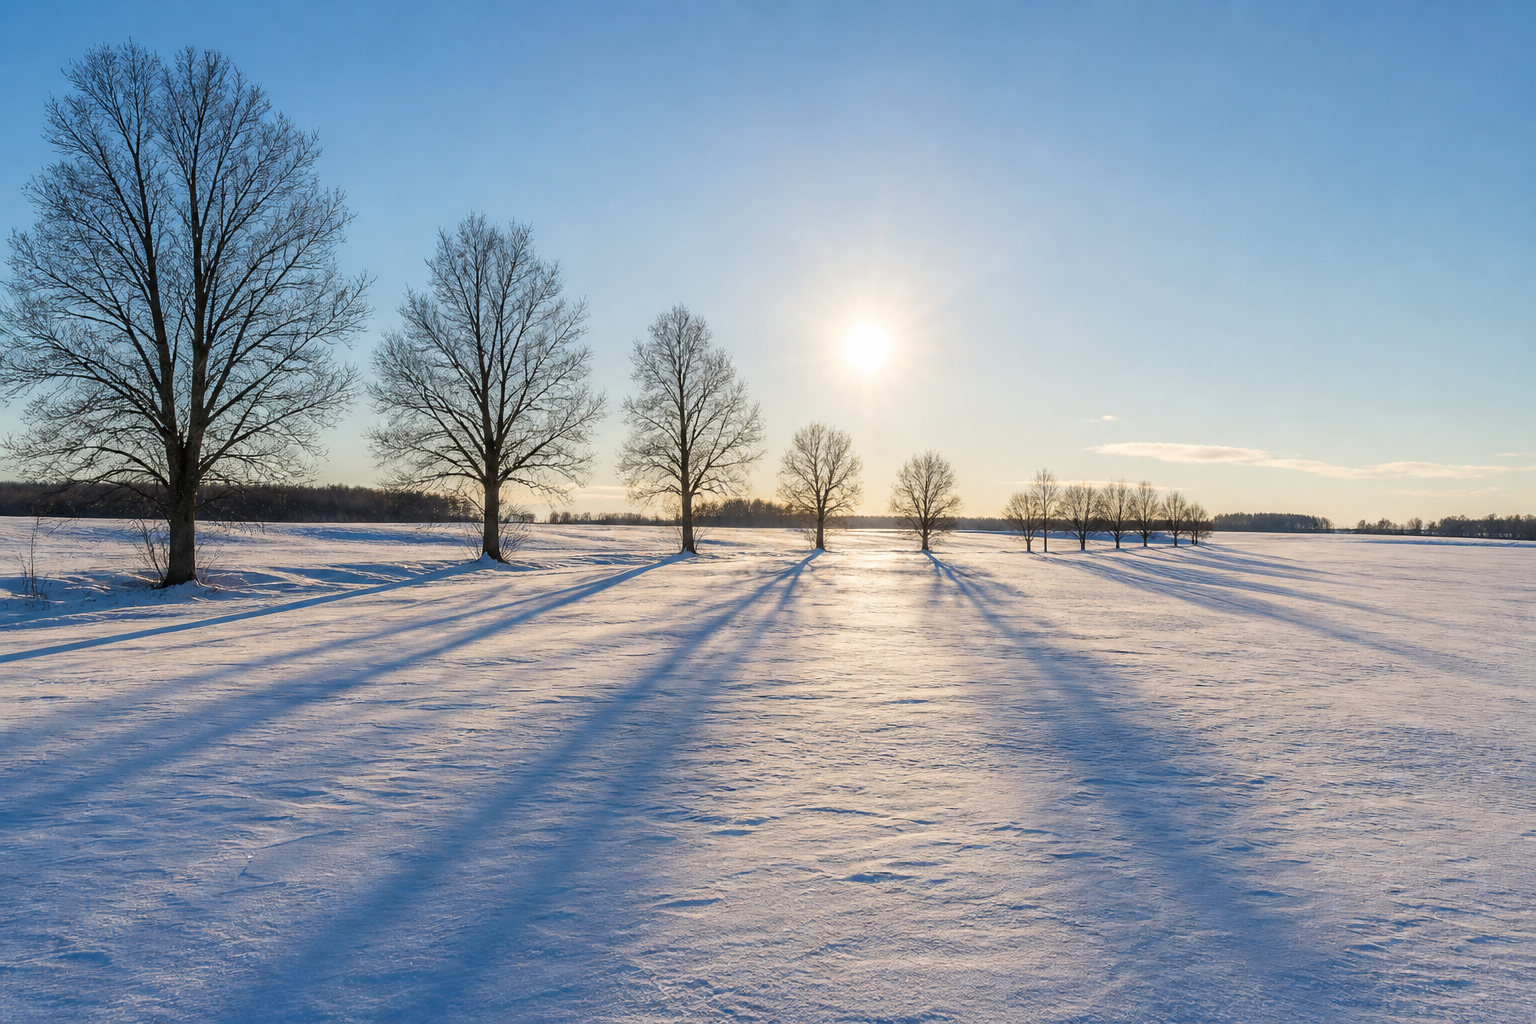
\includegraphics[width=0.58\linewidth]{images/book1/ai/g3-seasons-winter-sun.png}

{\small Un midi d'hiver~: le Soleil reste bas, la \omterm{def:g1:light-and-shadows:source}{lumière} arrive de biais, et les \omterm{def:g1:light-and-shadows:shadow}{ombres} s'allongent sur la neige.}
\end{omfigure}

\section{Exercices}

\begin{exercise}[$\star$]\label{exo:g3:sun-days-seasons:1}
En quelle \omterm{def:g3:sun-days-seasons:year}{saison} l'arc du Soleil est-il le plus haut et le plus
long~? Le plus bas et le plus court~? Quel effet cela a-t-il sur la
longueur de la journée~?
\end{exercise}

\begin{exercise}[$\star$]\label{exo:g3:sun-days-seasons:2}
À quel moment de la journée l'\omterm{def:g1:light-and-shadows:shadow}{ombre} d'un poteau est-elle la plus
courte~? Qu'a encore de particulier l'\omterm{def:g1:light-and-shadows:shadow}{ombre} de midi, jour après
jour~?
\end{exercise}

\begin{exercise}[$\star$]\label{exo:g3:sun-days-seasons:3}
Le même poteau jette à midi une \omterm{def:g1:light-and-shadows:shadow}{ombre} de $2$ longueurs de botte en
juin et de $7$ bottes en décembre. Explique la différence avec les
deux routes du Soleil.
\end{exercise}

\begin{exercise}[$\star$]\label{exo:g3:sun-days-seasons:4}
Comment un \omterm{def:g3:sun-days-seasons:sundial}{cadran solaire} donne-t-il l'heure~? De quoi son aiguille
mobile est-elle faite~?
\end{exercise}

\begin{exercise}[$\star$]\label{exo:g3:sun-days-seasons:5}
Dans \cref{met:g3:sun-days-seasons:build}, pourquoi le bâton
doit-il rester à un endroit ensoleillé toute la journée~? Qu'advient-il
de l'horloge par temps nuageux --- et la nuit~?
\end{exercise}

\begin{exercise}[$\star$]\label{exo:g3:sun-days-seasons:6}
Combien de temps la Terre met-elle pour faire un tour autour du
Soleil~? Combien de \omterm{def:g3:sun-days-seasons:year}{saisons} tiennent dans un tour~? Range-les dans
l'ordre, en partant du printemps.
\end{exercise}

\begin{exercise}[$\star$]\label{exo:g3:sun-days-seasons:7}
Combien de jours y a-t-il à peu près dans une année~? Et --- d'après
un chapitre précédent --- combien d'\omterm{ex:g2:measuring-time:clock}{heures} dans une journée~? Quel
voyage de la Terre produit chacun des deux~?
\end{exercise}

\begin{exercise}[$\star$]\label{exo:g3:sun-days-seasons:8}
Cite deux indices, visibles de ta fenêtre en une seule semaine, qui
te disent si tu es en plein été ou en plein hiver sans calendrier.
\end{exercise}

\begin{exercise}[$\star$]\label{exo:g3:sun-days-seasons:9}
Quand c'est l'hiver chez toi, quelle \omterm{def:g3:sun-days-seasons:year}{saison} est-ce pour les enfants
de l'autre moitié de la Terre~? Que prouve cela au sujet de l'idée
«~l'hiver arrive parce que la Terre entière est plus loin du
Soleil~»~?
\end{exercise}

\begin{exercise}[$\star\star$]\label{exo:g3:sun-days-seasons:10}
Une jardinière plante les cailloux de son horloge d'\omterm{def:g1:light-and-shadows:shadow}{ombre} en mars. En
juin, l'\omterm{def:g1:light-and-shadows:shadow}{ombre} ne touche plus les cailloux aux \omterm{ex:g2:measuring-time:clock}{heures} marquées. Le
bâton a-t-il bougé~? Explique ce qui a dérivé, à l'aide de
\cref{ex:g3:sun-days-seasons:shadowlength}.
\end{exercise}

\begin{exercise}[$\star\star$]\label{exo:g3:sun-days-seasons:11}
Une exploratrice se réveille sans montre ni téléphone, voit le Soleil
exactement au plus haut, et une heure plus tard trouve l'\omterm{def:g1:light-and-shadows:shadow}{ombre} de sa
tente déjà plus longue que la tente n'est haute. Vers quelle heure
s'est-elle réveillée, à peu près, et est-elle plus proche du plein
été ou du plein hiver~? Argumente à partir de la règle de midi et de
la longueur de l'\omterm{def:g1:light-and-shadows:shadow}{ombre}.
\end{exercise}
